\documentclass[tikz,border=10pt]{standalone}
\usepackage{amsmath,amssymb}
\usepackage[T1]{fontenc}
\usetikzlibrary{arrows.meta,positioning,fit,backgrounds,shadows.blur}

\begin{document}

% Figure 1: current PURE architecture
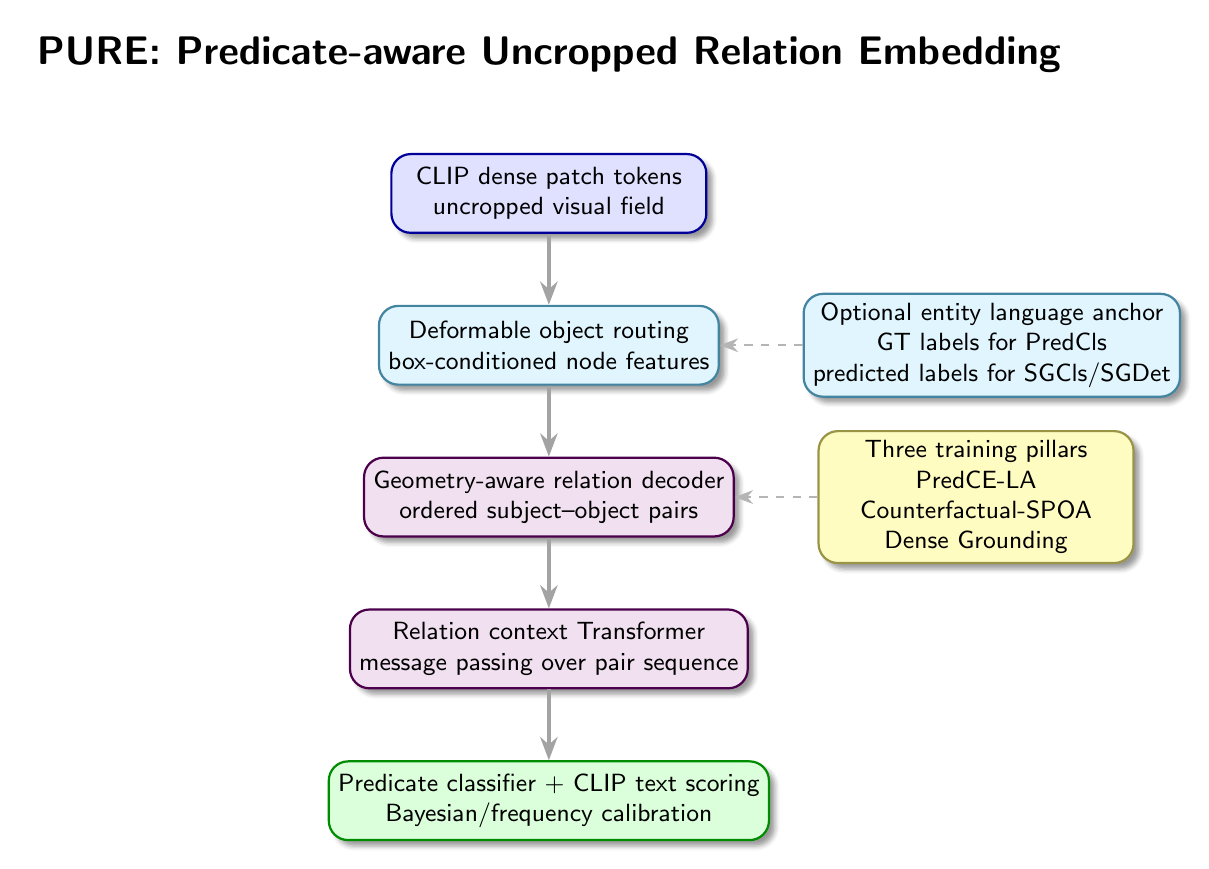
\begin{tikzpicture}[
  font=\sffamily,
  >=Stealth,
  node distance=0.9cm and 1.05cm,
  title/.style={font=\sffamily\bfseries\Large, align=center},
  block/.style={rectangle, rounded corners=7pt, draw=gray!65, fill=white, thick, blur shadow, minimum width=40mm, minimum height=10mm, align=center, font=\sffamily\small},
  vision/.style={block, fill=blue!12, draw=blue!60!black},
  nodeblk/.style={block, fill=cyan!12, draw=cyan!60!black},
  rel/.style={block, fill=violet!12, draw=violet!60!black},
  outputblk/.style={block, fill=green!14, draw=green!55!black},
  aux/.style={block, fill=yellow!24, draw=yellow!55!black},
  arrow/.style={->, very thick, draw=gray!72},
  soft/.style={->, thick, dashed, draw=gray!58}
]
\node[title] (title) {PURE: Predicate-aware Uncropped Relation Embedding};
\node[vision, below=0.9cm of title] (clip) {CLIP dense patch tokens\\uncropped visual field};
\node[nodeblk, below=of clip] (router) {Deformable object routing\\box-conditioned node features};
\node[nodeblk, right=of router] (anchor) {Optional entity language anchor\\GT labels for PredCls\\predicted labels for SGCls/SGDet};
\node[rel, below=of router] (pair) {Geometry-aware relation decoder\\ordered subject--object pairs};
\node[rel, below=of pair] (ctx) {Relation context Transformer\\message passing over pair sequence};
\node[outputblk, below=of ctx] (score) {Predicate classifier + CLIP text scoring\\Bayesian/frequency calibration};
\node[aux, right=of pair] (loss) {Three training pillars\\PredCE-LA\\Counterfactual-SPOA\\Dense Grounding};
\draw[arrow] (clip) -- (router);
\draw[arrow] (router) -- (pair);
\draw[arrow] (pair) -- (ctx);
\draw[arrow] (ctx) -- (score);
\draw[soft] (anchor) -- (router);
\draw[soft] (loss) -- (pair);
\end{tikzpicture}

\vspace{8mm}

% Figure 2: curriculum
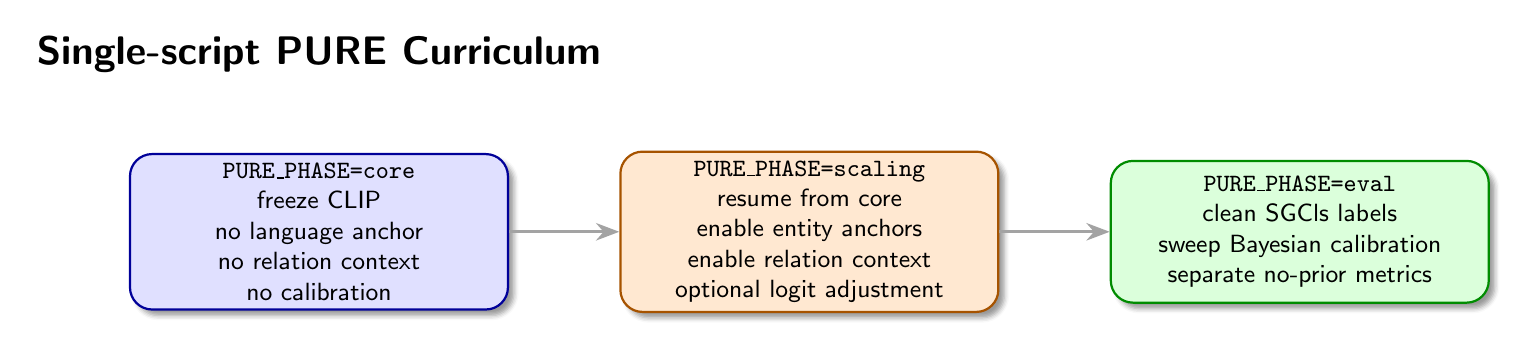
\begin{tikzpicture}[
  font=\sffamily,
  >=Stealth,
  node distance=1.0cm and 1.4cm,
  title/.style={font=\sffamily\bfseries\Large, align=center},
  stage/.style={rectangle, rounded corners=8pt, draw=gray!65, fill=white, thick, blur shadow, minimum width=48mm, minimum height=18mm, align=center, font=\sffamily\small},
  core/.style={stage, fill=blue!12, draw=blue!60!black},
  scaling/.style={stage, fill=orange!18, draw=orange!65!black},
  eval/.style={stage, fill=green!14, draw=green!55!black},
  arrow/.style={->, very thick, draw=gray!72}
]
\node[title] (title) {Single-script PURE Curriculum};
\node[core, below=0.9cm of title] (core) {\texttt{PURE\_PHASE=core}\\freeze CLIP\\no language anchor\\no relation context\\no calibration};
\node[scaling, right=of core] (scaling) {\texttt{PURE\_PHASE=scaling}\\resume from core\\enable entity anchors\\enable relation context\\optional logit adjustment};
\node[eval, right=of scaling] (eval) {\texttt{PURE\_PHASE=eval}\\clean SGCls labels\\sweep Bayesian calibration\\separate no-prior metrics};
\draw[arrow] (core) -- (scaling);
\draw[arrow] (scaling) -- (eval);
\end{tikzpicture}

\vspace{8mm}

% Figure 3: CORE status
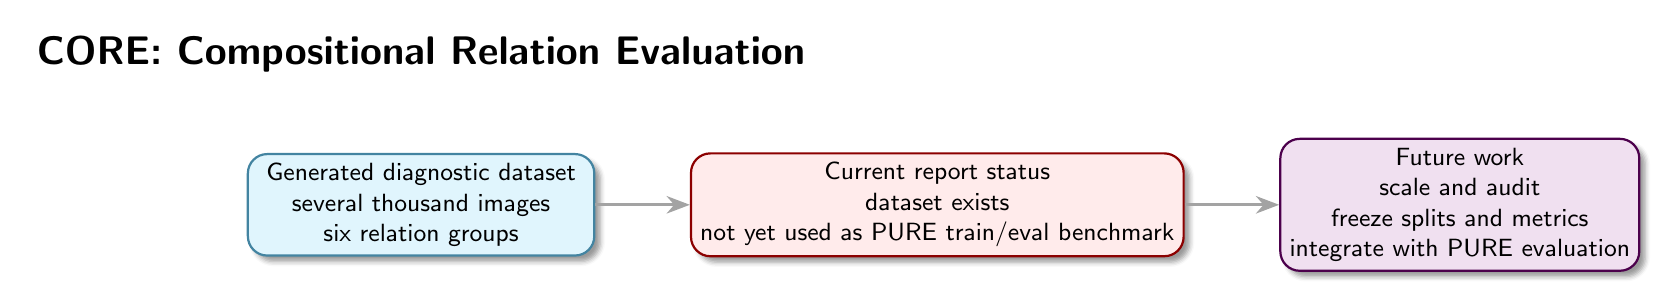
\begin{tikzpicture}[
  font=\sffamily,
  >=Stealth,
  node distance=0.9cm and 1.2cm,
  title/.style={font=\sffamily\bfseries\Large, align=center},
  block/.style={rectangle, rounded corners=7pt, draw=gray!65, fill=white, thick, blur shadow, minimum width=44mm, minimum height=12mm, align=center, font=\sffamily\small},
  data/.style={block, fill=cyan!12, draw=cyan!60!black},
  future/.style={block, fill=violet!12, draw=violet!60!black},
  warn/.style={block, fill=red!8, draw=red!55!black},
  arrow/.style={->, very thick, draw=gray!72}
]
\node[title] (title) {CORE: Compositional Relation Evaluation};
\node[data, below=0.9cm of title] (data) {Generated diagnostic dataset\\several thousand images\\six relation groups};
\node[warn, right=of data] (status) {Current report status\\dataset exists\\not yet used as PURE train/eval benchmark};
\node[future, right=of status] (future) {Future work\\scale and audit\\freeze splits and metrics\\integrate with PURE evaluation};
\draw[arrow] (data) -- (status);
\draw[arrow] (status) -- (future);
\end{tikzpicture}

\end{document}
